\documentclass[11pt]{article}
\usepackage[utf8]{inputenc}
\usepackage[T1]{fontenc}
\usepackage{amsmath}
\usepackage{amsfonts}
\usepackage{amssymb}
\usepackage[version=4]{mhchem}
\usepackage{stmaryrd}
\usepackage{graphicx}
\usepackage[export]{adjustbox}
\graphicspath{ {./images/} }

\begin{document}
Natural Resources Other Than Land

Real assets are economic resources that create or add to the consumption opportunities available to people. All consumption ultimately originates from real assets.

Financial assets are the counterpart to real assets. Financial assets serve as conduits of value rather than as direct creators of consumption opportunities.

This session discusses institutional-quality investments in two types of real assets: natural resources and land. Natural resources are real assets that have received no or almost no human alteration. Commodities are often categorized as natural resources, but since they are typically processed or otherwise altered, they are discussed in later session. Undeveloped land and timberland are almost always classified as natural resources. This session concludes with a discussion of the challenges raised in examining past return data when valuations are based on appraisals rather than market prices.

Examples of natural resources include oil, natural gas, coal, ore, land, water, wind, and other inputs to production that largely remain in a natural state and location. Most natural resources are related to facilitating energy consumption because energy is such a major input to the world economy. For example, energy consumption tends to represent approximately $8 \%$ to $10 \%$ of gross domestic product in the United States. Other substantial sectors of natural resources include land and metal ores and other minerals.

\section*{Economic Roles and Vehicles of Natural Resources}
A large portion of natural resources is under the earth's surface. In most jurisdictions, private land ownership is limited to surface rights, with the ownership of underground mineral and energy rights retained by governments. However, in the United States, private land ownership has typically included mineral rights. Although much U.S. land is publicly owned, some states allow split estates. A split estate is when surface rights and mineral rights are separately owned.

Public or private owners of natural resources often lease their natural resource rights to developers for eventual extraction. Thus, effective economic ownership of a natural resource is often accomplished through the purchase or leasing of rights rather than through transfer of recorded property ownership.

Pure plays on a private investment in natural resources are rare. A pure play on an investment is an investment vehicle that offers direct exposure to the risks and returns of a specific type of investment without the inclusion of other exposures. Since most underground natural resources are not privately owned and most U.S. privately owned natural resources are commingled with surface rights, there are few institutional-quality investments with returns determined almost solely by the values of the underlying natural resources.

An example of a somewhat pure play on natural resources is Natural Resource Partners L.P., which might also be viewed as a liquid alternative. Natural Resource Partners L.P. is an MLP (master limited partnership) that trades on the NYSE under the ticker symbol NRP. (MLP structures were introduced in the session, The Environment of Alternative Investments). NRP is principally engaged in owning and managing mineral reserve properties including coal, aggregates, and oil and gas reserves across the United States. Its performance over the financial crisis tended to follow the overall market, while its performance since then has been linked to the prospects for profits from its coal properties. This highlights the challenge of using public markets to access pure plays on natural resources. As is discussed later in this session, the lack of such publicly-traded investment opportunities limits the evidence available from observing market prices on natural resource investments.

In summary, institutional ownership of natural resources can be achieved through land ownership that includes underground rights, ownership of mineral rights, or leasing of mineral rights. There are some opportunities for pure plays on natural resources through private partnerships or listed partnerships (MLPs); however, most global natural resources are either owned by governments or leased to operating firms.

\section*{Natural Resources as Exchange Options}
Viewing natural resources as options to develop commodities and other real assets offers important insight regarding the analysis of natural resources. A potential developer of a natural resource anticipates expending money to develop the natural resource into a commodity or another improved real asset just as a call option holder anticipates expending cash to acquire an asset. However, an essential element of natural resources as options is that the amount of money necessary to develop the resources is uncertain. Therefore, a key aspect of natural resources as options is that they are better analyzed as an exchange option rather than as a call option with a fixed strike price. An exchange option is an option to exchange one risky asset for another rather than to buy or sell one asset at a fixed exercise or strike price.

The process of developing a resource involves using the mineral rights along with fuel, materials, labor, management, and equipment to bring a commodity to market. It is for this reason that a natural resource should be viewed as an exchange option in which the developer exchanges one set of resources with stochastic prices (the production inputs) to obtain the output (with a price that is also stochastic).

For example, a firm that owns mineral rights to gold ore can be viewed as owning an option to exchange the mineral rights, fuel, mining equipment, labor, management, and materials necessary to extract the gold for a long position in the underlying gold, as depicted more generally in the next exhibit, Receivables and Deliverables in Exchange Option.

\begin{center}
\begin{tabular}{|ll|}
\hline
Receivables & Deliverables \\
\hline
Processed minerals (e.g., gold) & Mineral rights (e.g., mining rights), fuel, equipment, labor, management, materials \\
\hline
\end{tabular}
\end{center}

The market prices of both the receivables and the deliverables change. As discussed in the session Derivatives and Risk-Neutral Valuation, like all options, the value of an exchange option depends on volatility. In the case of an exchange option, the volatility depends on (1) the volatility of the price of the asset(s) being delivered, (2) the volatility of the price of the asset(s) being received, and (3) the covariance or correlation coefficient between the prices.

The volatility underlying the exchange option adheres to the familiar formula of Markowitz, which defines the volatility of a two-asset portfolio as depending on both the individual volatilities of the assets and their correlation. If the cost of development is highly correlated with the value of the commodity, the volatility of the value of the exchange will be lower and the value of the option will be lower (everything else being equal). The option can be especially valuable when development costs and commodity prices are not highly positively correlated.

The prices of developing a resource can change due to technological advances and other factors, such as environmental and regulatory concerns. Recent technological breakthroughs in drilling for oil and gas (e.g., hydraulic fracturing, or fracking) have enabled development of resources previously deemed economically infeasible. The transformation of previously worthless shale oil formations into highly valuable producing wells is an illustration of the importance of volatility in development costs that are uncorrelated with commodity prices.

\section*{Moneyness as a Crucial Factor in Natural Resource Development}
The next exhibit illustrates a value diagram for natural resource development as an option that is similar to the value diagram of a call option. However, there is an important distinction between the diagram in the exhibit Natural Resource Development as a Call Option and the diagram of a traditional call option (shown in the session Derivatives and Risk-Neutral Valuation). The horizontal axis of the next exhibit is the ratio of the current price of the developed natural resource to the current cost of development. The key idea is that both the price of the developed natural resource and the cost of developing the resource are stochastic, so the moneyness depends on the spread between the benefits and the costs of development.

\begin{center}
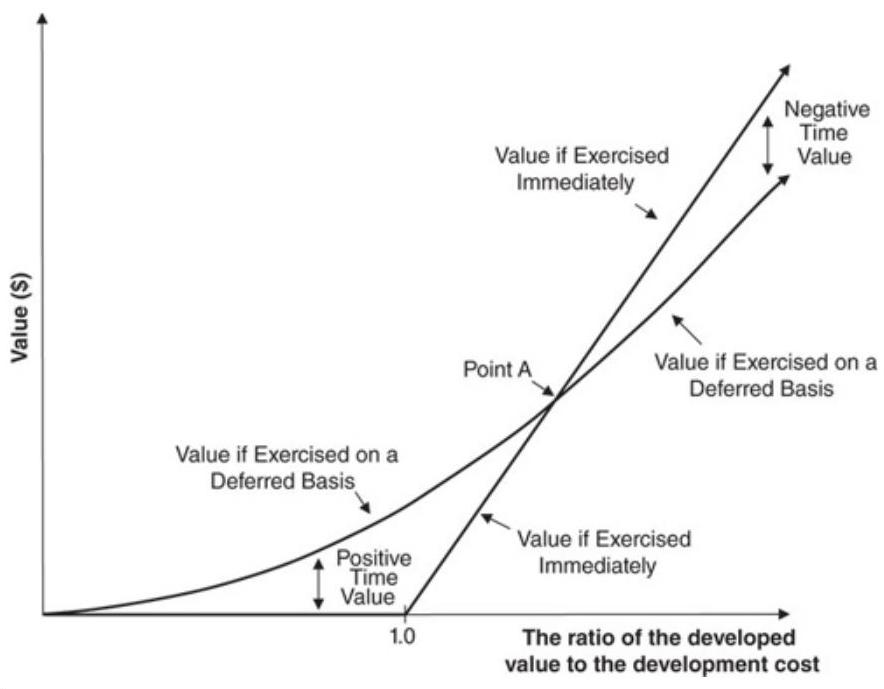
\includegraphics[max width=\textwidth]{2024_04_10_c7d72f7af63ea46ad391g-3}
\end{center}

\section*{Natural Resource Development as a Call Option}
Moneyness in the exhibit, Natural Resource Development as a Call Option reflects the direct benefit-to-cost ratio of developing the natural resource immediately. The exhibit above has three ranges of moneyness: in-the-money (to the right of 1.0 on the horizontal axis), at-the-money (1.0 on the horizontal axis), and out-of-themoney (to the left of 1.0 on the horizontal axis). Being in-the-money means that if the mineral rights are mined at the current price of the commodity (e.g., gold), then the revenues from the sale of the commodity will exceed the current costs of developing the commodity (i.e., mineral rights, fuel, labor, management, materials, and equipment).

The option to develop rights to a natural resource may have no expiration date or may be leased on a temporary basis. We examine here the case of a perpetual option. A perpetual option is an American option with no expiration date. All perpetual options are American options, since a European perpetual option could never be exercised and therefore would have no value.

In traditional option theory, most options should be held until expiration. There are limited cases in which an option should be exercised early, such as deep-in-themoney put options and call options prior to ex-dividend dates. Since the option to develop a natural resource is generally a perpetual option, the critical issue is how the owner makes the decision of when to exercise the option.

A natural resource should generally not be developed until the option is substantially into the money. But how far into the money should the option be to justify it being exercised?

Consider the following scenario: A tract of land has moderate quantities of ore containing gold. Suppose that at a market price of $\$ 1,500$, the gold can be mined at a cost of $\$ 1,400$ per ounce, for a profit of $\$ 100$ per ounce. Does it make sense to mine the gold now because of the positive time value of money? The answer is that it depends on three things: the volatility in the price of gold, the volatility in the cost of mining the gold, and the correlation between the two.

\section*{Moneyness Differences and Natural Resource Development}
The exhibit, Natural Resource Development as a Call Option illustrates a key insight into natural resource development when the moneyness depicted on the horizontal axis is viewed as representing different properties. Different properties containing natural resources have different benefit-to-cost ratios from development. Returning to the gold example, consider two properties: (1) a property in a jurisdiction supportive of development, with easily accessible material that is rich in gold ore, and (2) a property subject to strict environmental regulations, and poorly accessible material with low concentrations of gold ore. Obviously the first property reflects a development option that is deep in-the-money, whereas the second property reflects a development option that is deep out-of-the-money.

Common sense indicates that the first property should be developed before the second property. In economics, this is known as the low-hanging-fruit principle. The low-hanging-fruit principle states that the first action that should be taken is the one that reaps the highest benefits over costs. Thus, the order in which natural resource properties are developed should tend to be driven by the low-hanging-fruit principle.

\section*{Why Some In-the-Money Options Should Not Be Exercised Immediately}
Option theory guides the distinction between the properties that are sufficiently in-the-money to justify immediate development and the properties for which development should be postponed awaiting subsequent price changes.

The value of delaying a decision to exercise an in-the-money development option, as in all in-the-money options, is based on the time value of money and an analysis of the benefit of awaiting further information. The convex nature of the payoff diagram in the previous exhibit illustrates the asymmetric payoff to options. A long position in an option has increased value at an increasing rate in one direction (in the case of the exhibit, Natural Resource Development as a Call Option, moving to the right) and decreased value at a decreasing rate in the other direction. The essence of this convexity to holders of long positions in options is to consider the advantage generated by the volatilities of market prices when deciding on the optimal time to exercise an option.

To illustrate, consider a perpetual option with a current intrinsic value of $\$ 100$. An intrinsic option value is the greater of $\$ 0$ and the value of an option if exercised immediately. Assume that the option's owner believes that future changes in the moneyness of the option are random and, for simplicity, are symmetric. If the moneyness of the option grows substantially higher by increments of, say, $\$ 200$, then the option's intrinsic value will rise to $\$ 300$. But if the moneyness falls by the same amount ( $\$ 200$ ), the option's intrinsic value will not fall to $-\$ 100$; it can only fall to $\$ 0$.

These numbers illustrate why the owner of the option should be reluctant to exercise the option. If the owner exercised the option now, it would be worth $\$ 100$. But the owner might very well prefer a $50 \%$ chance of receiving $\$ 300$ and a $50 \%$ chance of having an out-of-the-money option that might become valuable someday.

In this simplified analysis, the option should not be exercised until the time value of the option is zero. The time value of an option is the excess of an option's price above its intrinsic value. The sum of an option's intrinsic value and its time value is equal to the option's total value (or price), as depicted in Equation 1:


\begin{equation*}
\text { Option Price or Value }=\text { Intrinsic Option Value }+ \text { Time Value of Option } \tag{1}
\end{equation*}


Returning to the exhibit Natural Resource Development as a Call Option, the point at and above which a development option should be exercised is depicted by point A, where the time value of the option is zero. Above that point, the developer gains more wealth from immediately reaping the profit of development than from delaying the decision to exercise the option and potentially benefit from the option's convexity and stochastic market prices. The financial economics are similar to the decision to exercise an American put option early.

From a macroeconomic perspective, the price of the associated commodity rises or falls to either increase or decrease development rates so that the supply of the commodity matches the demand for the commodity.

\section*{Implications of Moneyness for Risk of Natural Resources}
The exhibit, Natural Resource Development as a Call Option and the related discussions provide insight into the risks of natural resources. For natural resources that represent in-the-money development options, the short-term financial risks are primarily driven by the price of the underlying commodity. The steep slope of the option curve in Natural Resource Development as a Call Option exhibit for options that are far in-the-money indicates that changes in the price of the commodity are the dominant source of short-term volatility in the value of the option to develop the natural resource. Higher moneyness shortens the time horizon of the exercise of the option and reduces the chance that the option's price will be substantially altered directly by changes in the costs of developing the natural resource.

Conversely, natural resources that represent out-of-the-money development options have substantial sensitivity to uncertainty other than the price of the underlying commodity. The more distant time horizon for possible development increases the sensitivity of the natural resource's price to changes in development costs, interest rates, and other factors.


\end{document}